
\section{wnlrt -Weakly Non Linear Ray Tracing}
\label{sec: wnlrt}

{\bf wnlrt} is a non-linear geometrical acoustics program that calculates the second order (weak shock theory) transport equation along a ray path. The program requires geometrical acoustics input. In particular, the ray path and the linear amplitudes (the Jacobean for the transformation from cartesian to ray coordinates) must be provided by the user as input. The algorithm uses a spilt step approach in which the ray path is traversed in small steps. Non-linear effects are treated in the time domain in each step. The solution is then transformed to the frequency domain where atmospheric attenuation is applied. 

\subsection{Mathematical Background}
\label{sec: wnlrt math}

{\bf {wnlrt}} uses a weakly non-linear ray tracing algorithm (the original code was developed by Joel B. Lonzaga) to propagate a signal from an impulsive source to a receiver through a range dependent 3-d atmosphere with winds. For the theory and algorithm refer to
reference~\cite{non-lin_therm}. 

\subsection{Running wnlrt}
\label{sec: running wnlrt}

{\bf wnlrt} is not a stand-alone program but requires input from a geometrical acoustics program. The required data and file format is detailed in the help page provided by the program and reproduced below. A modified version of Philip Blom's {\bf GeoAc-v1.1.1}, called {\bf GeoAc-v1.1.1-ncpaprop}, is provided. It is identical to {\bf GeoAc1.1.1} with the exception that it outputs ray files with the information and in the format required by {\bf wnlrt}. The executables generated by compiling {\bf GeoAc-v1.1.1-ncpaprop} are named \verb+prog-ncpaprop+ where \verb+prog+ is the original name of the executable. 

Making sure that the executable for {\bf wnlrt} is in the system's path, it can be run by entering 
\begin{verbatim} 
    wnlrt [--option1 val1] [--option2 val2] [...] [--flag1] [...] 
\end{verbatim}
on a command line. Generally, options are followed by values, either numbers, strings or filenames. Flags are not. Entering \verb"wnlrt" without any options or flags sends the following help page to the screen: 

\begin{verbatim}
This code uses a weakly non-linear ray tracing algorithm to propagate a signal
from an impulsive source to a receiver through a stratified atmosphere with 
winds. For the theory and algorithm refer to: 
Joel B. Lonzaga, Roger M. Waxler, Jelle D. Assink and Carrick L. Talmadge,
"Modeling waveforms of infrasound arrivals from impulsive sources using 
weakly non-linear ray theory", Geophys. J. Int. (2015) 200, 1337-1361.

Usage: 
./wnlrt [--option1 val1] [--option2 val2] [--flag1] [...]

The options below can be specified at the command line or in a colon-separated
file "wnlrt.options". Command-line options override file options.
Be sure to precede all options with two minuses (--). The program options can
be of two kinds: pairs of [--option_name value] or flags. The values can be 
numbers or strings (arrays of characters). The flags do not take a value on the
command line; they are boolean switches signaling the program for a certain 
action to occur.

 --help -h            Print this message and exit

PREREQUISITE
This code requires the user to provide an eigenray file obtained from an external
ray-tracing package GeoAc1.1.1 authored by Phil Blom, currently at Sandia
National Lab, and whose work began at NCPA under the direction of Roger Waxler.
(As an example see the included ToyAtmo_Eigenray-0.dat file.)
The 15-column eigenray file has a 4-line header providing information about 
the source and receiver locations, the ray launch angles and the column names
as in the following example:
  Source Location (kilometers) : (0, 0, 0).
  Receiver Location (kilometers) : (350, 0, 0).
  theta = 18.0303, phi = 90,  c0(zground) = 0.340322 km/s
  # x [km]  y [km]  z [km]  Geo. Atten. [dB]  Atmo. Atten. [dB] Travel Time [s]
    rho [gm/cm^3]  c [km/s]  u [km/s]  v [km/s]  w [km/s]
    Slowness_x [s/km]  Slowness_y [s/km]  Slowness_z [s/km]  Jacobian [km^2/rad^2]

REQUIRED options:
 --eigenrayfile        Provide name of previously obtained eigenray file.
                       Currently this eigenray file is obtained by running
                       the modified version of GeoAc1.1.1 that outputs 
                       relevant parameters along the ray path.

OPTIONAL options [defaults]:
 --waveform            Provide the type of waveform at the source. 
                       Can be Nwave or pulse [Nwave]. 
 --ampl                Provide the initial pressure waveform amplitude. [1 Pa]
 --duration            Provide the initial waveform duration [0.5 secs]

OUTPUT text files:
 ray_params.dat
                       Contains ray info and acoustic pressure [Pa]; 6 columns 
                       [ x, y, z, raypath_length, travel_time, acoustic pressure ]

 pressure_wf_evolution.dat
                       Stores N pressure waveforms at N time steps along the ray.
                       The pressure units are Pascals.
                       The file contains (N+1) columns in the following order: 
                       [ reduced_time, pressure waveform_at_step_1 ...
                       [ pressure waveform_at_step_2 ... waveform_at_step_N ]

 final_waveform_spectrum.dat
                       Stores waveform spectrum at the ray's end point 
                       Contains 3 columns: [ frequency, real part, imag part ]

QUICK-START EXAMPLES:
./wnlrt --eigenrayfile ToyAtmo_Eigenray-0.dat
./wnlrt --eigenrayfile ToyAtmo_Eigenray-0.dat --waveform Nwave --ampl 500 --duration 0.5
\end{verbatim}

\subsection{Running wnrt: example}

Here is a simple example run to illustrate the main input for \verb+wnlrt+.
\begin{verbatim} 
    ./wnlrt --eigenrayfile ToyAtmo_Eigenray-0.dat
\end{verbatim}

\begin{figure}[h]
\begin{center}
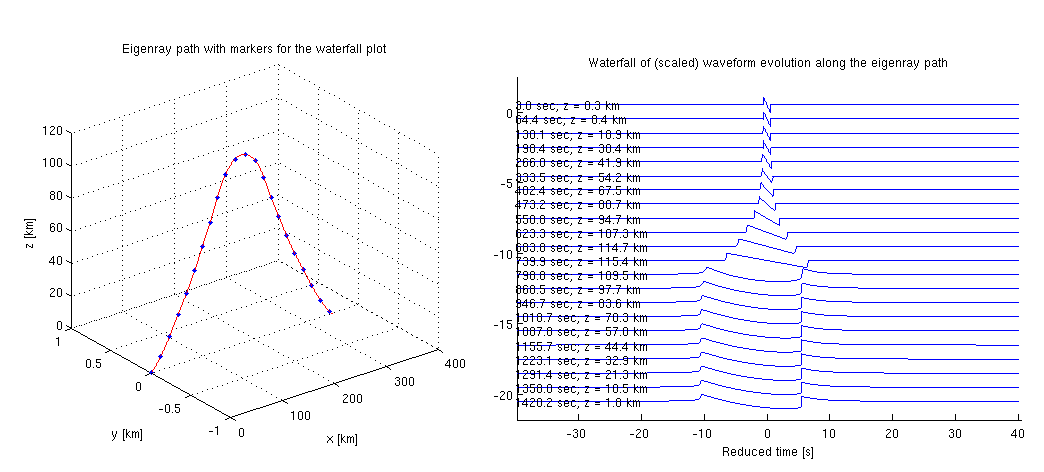
\includegraphics[scale=0.45,trim = 40 10 10 20,clip]{figs/fig_wnrt_example.png}
\end{center}
\caption{N-wave waveform evolution along a raypath.}
\label{fig:wnlrt_fig1}
\end{figure}

This example is for of an N-wave of unit amplitude and 0.5 second duration along a raypath defined in file ToyAtmo\_Eigenray-0.dat. The raypath is shown in the left panel in Figure \ref{fig:wnlrt_fig1} . In the right panel a waterfall of the (scaled) N-wave evolution is presented at various points on the raypath. It illustrates the non-linear effect of propagation: the N-wave stretches gradually and "softens" in frequency content due to absorption in the air. 

The actual eigenray files to be used with this module are obtained from a modification of external ray-tracing package GeoAc1.1.1  author and maintained by Phil Blom, currently at Los Alamos National Laboratory. The modification is called GeoAc1.1.1-ncpaprop and is included with the ncpaprop package. The eigenray file is a 15-column text file whose format is described in the {\bf wnlrt} help page reproduced above.



